\chapter{Green's function}
\label{2011-m-gf}

This chapter is the beginning of a series of chapters dealing with the solution of differential equations related to theoretical physics.
\index{differential equation}
These differential equations are {\em linear}; that is, the ``sought after'' function $\Psi (x), y(x), \phi (t)$ {\it et cetera}
occur only as a polynomial of degree zero and one, and {\em not} of any higher degree, such as, for instance, $[y(x)]^2$.

\section{Elegant way to solve linear differential equations}

Green's functions present a very elegant way of solving linear differential equations
of the form
\begin{equation}
\begin{split}
{\cal L}_x y(x)=   f(x) \textrm{, with the differential operator}\\
{\cal L}_x =
a_n (x)\frac{d^n}{dx^n} +
a_{n-1} (x)\frac{d^{n-1}}{dx^{n-1}} +
\ldots
+
a_1 (x)\frac{d}{dx}
+
a_0 (x) \\
\qquad = \sum_{j=0}^n  a_j(x) \frac{d^j}{dx^j} ,
\end{split}
\label{2011-m-egfp}
\end{equation}
where $a_i(x)$, $0\le i \le n$ are functions of $x$.
The idea of the Green's function method is quite straightforward:
if we are able to obtain the ``inverse'' $G$ of the differential operator  ${\cal L}$ defined by
\begin{equation}
{\cal L}_x G(x,    x'   )=   \delta (x-    x'   ),
\label{2011-m-egfp01}
\end{equation}
with  $\delta$ representing Dirac's delta function, then the solution to the inhomogeneous differential
equation   (\ref{2011-m-egfp}) can be obtained by integrating  $G(x,x')$ alongside with
\index{inhomogeneous differential equation}
the inhomogeneous term $f(    x'   )$; that is, by forming
\begin{equation}
\begin{split}
y(x) = \int_{-\infty}^\infty
G(x,    x'   )
f(    x'   )
d     x'   .
\end{split}
\label{2011-m-egfp1}
\end{equation}
This claim, as posted in Eq. (\ref{2011-m-egfp1}),
can be verified by explicitly applying the differential operator  ${\cal L}_x$
to the solution $y(x)$,
\begin{equation}
\begin{split}
{\cal L}_x y(x)\\
\qquad  =
{\cal L}_x \int_{-\infty}^\infty
G(x,    x'   )
f(    x'   )
d     x'        \\
\qquad  =
\int_{-\infty}^\infty
{\cal L}_x G(x,    x'   )
f(    x'   )
d     x'      \\
\qquad  =
\int_{-\infty}^\infty
\delta (x-    x'   )
f(    x'   )
d     x'      \\
\qquad  =
f(x)  .
\end{split}
\label{2011-m-egfp12}
\end{equation}

{
\color{blue}
\bexample

Let us check whether
$G(x,x')=H (x-x')\sinh (x-x')$
is a Green's function of the differential operator ${\cal L}_x={d^2\over dx^2}-1$.
In this case, all we have to do is to verify that   ${\cal L}_x$, applied to $G(x,x')$, actually renders $\delta (x-x')$,
as required by Eq. (\ref{2011-m-egfp01}).

\begin{equation}
\begin{split}
   {\cal L}_xG(x,x')=\delta(x-x')\\
   \left({d^2\over dx^2}-1\right)H(x-x')\sinh(x-x')
   \stackrel{?}{=} \delta(x-x')
\end{split}
\end{equation}
Note that $\frac{d}{dx}\sinh x=\cosh x$,
and ${d\over dx}\cosh x=\sinh x$; and hence
$$
   {d\over dx}\left(\underbrace{\delta(x-x')\sinh(x-x')}_{\mbox{$=0$}}
   +H(x-x')\cosh(x-x')\right)-H(x-x')\sinh(x-x')=
$$
$$
   \underbrace{\delta(x-x')\cosh(x-x')}_{=\delta(x-x')} + H (x-x')\sinh(x-x')-H (x-x')\sinh(x-x')=
   \delta(x-x').
$$
\eexample
}

\section{Nonuniqueness of solution}

The solution (\ref{2011-m-egfp12}) so obtained is {\em not unique}, as it is only a special solution to the inhomogeneous
equation (\ref{2011-m-egfp}).
The general solution to (\ref{2011-m-egfp}) can be found
by adding the general solution $y_0(x)$
of the corresponding {\em homogeneous} differential equation
\index{homogeneous differential equation}
\begin{equation}
\begin{split}
{\cal L}_x y_0(x)=   0
\end{split}
\label{2011-m-egfp0}
\end{equation}
to one special solution -- say, the one obtained in Eq. (\ref{2011-m-egfp12}) through Green's function techniques.

{\color{OliveGreen}
\bproof
Indeed,  the most general solution
\begin{equation}
Y(x)  = y(x) + y_0(x)
\label{2011-m-egfpgs}
\end{equation}
clearly is a solution of the inhomogeneous differential equation (\ref{2011-m-egfp12}),
as
\begin{equation}
{\cal L}_x Y(x)  ={\cal L}_x y(x) + {\cal L}_x y_0(x) =f(x)+0 =f(x).
\label{2011-m-egfpgs2}
\end{equation}

Conversely, any two distinct special solutions $y_1(x)$ and $y_2(x)$ of the inhomogeneous differential equation (\ref{2011-m-egfp12})
differ only by a function which is a solution of the homogeneous differential equation (\ref{2011-m-egfp0}), because
due to linearity of ${\cal L}_x$, their difference
$y_1(x) - y_2(x)$ can
be parameterized by some function $y_0$   which is the solution of the homogeneous differential equation:
\begin{equation}
{\cal L}_x [y_1(x) - y_2(x)]  ={\cal L}_x y_1(x) + {\cal L}_x y_2(x) =f(x) -f(x) =0.
\label{2011-m-egfpgs3}
\end{equation}

\eproof
}

\section{Green's functions of translational invariant differential operators}

From now on, we assume that the coefficients $a_j(x) =a_j$
in Eq. (\ref{2011-m-egfp}) are constants, and thus are {\em translational invariant}.
Then the differential operator ${\cal L}_x$, as well as the entire {\it Ansatz} (\ref{2011-m-egfp01})
for   $G(x,x')$, is translation invariant,
because derivatives are defined only by relative distances, and $\delta (x-x')$
is translation invariant for the same reason.
Hence,
\begin{equation}
G(x,x')= G(x-x').
\end{equation}
For such translation invariant systems, the Fourier analysis \index{Fourier analysis}
presents an excellent way of
analyzing the situation.

{\color{OliveGreen}
\bproof
Let us see why translanslation invariance of the coefficients
$a_j (x)=a_j(x+\xi )=a_j$
under the translation $x\rightarrow x + \xi $ with arbitrary $\xi $ --
that is, independence of the coefficients $a_j$ on the ``coordinate''
or ``parameter'' $x$ -- and thus of
the Green's function, implies a simple form of the latter.
Translanslation invariance of the Green's function really means
\begin{equation}
G(x+\xi ,x'+\xi )= G(x,x').
\end{equation}
Now set $\xi = - x'$; then we can define a new Green's function that just depends on
one argument (instead of previously two), which is the difference of the old arguments
\begin{equation}
G(x - x',x' - x')= G(x - x',0)\rightarrow G(x-x').
\end{equation}
\eproof
}

\section{Solutions with fixed boundary or initial values}

For applications, it is important to adapt the solutions of some inhomogeneous differential equation
to boundary and initial value problems.
\index{initial value problem}
\index{boundary value problem}
In particular, a properly chosen $G(x-    x'   )$, in its dependence on the parameter $x$, ``inherits''
some behavior of the solution $y(x)$.
Suppose, for instance, we would like to find solutions with $y(x_i)=0$
for some parameter values $x_i$, $i=1,\ldots ,k$.
Then, the Green's function $G$ must vanish there also
\begin{equation}
G(x_i-    x'   ) = 0  \textrm{ for } i=1,\ldots ,k.
\end{equation}

\section{Finding Green's functions by spectral decompositions}

It has been mentioned earlier
(cf. Section  \ref{2012-m-efed1} on page \pageref{2012-m-efed1})
that the  $\delta$-function
can be expressed in terms of various
{\em eigenfunction expansions}.
\index{eigenfunction expansion}
We shall make use of these expansions here \cite{duffy2001}.

Suppose $\psi_i(x)$ are
{\em eigenfunctions}
\index{eigenfunction}
of the differential operator ${\cal L}_x $,
and $\lambda_i$ are the associated {\em eigenvalues}; that is,
\index{eigenvalue}
\begin{equation}
{\cal L}_x \psi_i(x) =\lambda_i \psi_i(x).
\end{equation}
Suppose further that ${\cal L}_x$ is of degree $n$,
and therefore (we assume without proof)
that we know all (a complete set of) the $n$ eigenfunctions
$\psi_1(x), \psi_2(x), \ldots ,\psi_n(x)$ of ${\cal L}_x$.
In this case, orthogonality  of the system of eigenfunctions holds, such that
\begin{equation}
\int_{-\infty}^\infty \overline{\psi_i(    x    )}\psi_j(x)  dx =\delta_{ij} ,
\label{2011-m-egfcr1orthogon}
\end{equation}
as well as completeness, such that
\index{resolution of the identity}
\index{completeness}
\begin{equation}
\sum_{i=1}^n \overline{\psi_i( x' )}\psi_i(x) =\delta ( x - x')
.
\label{2011-m-egfcr1}
\end{equation}
$\overline{\psi_i(    x'   )}$ stands for the complex conjugate of ${\psi_i(    x'   )}$.
The sum in Eq. (\ref{2011-m-egfcr1}) stands for an integral in the case of continuous spectrum of  ${\cal L}_x $.
In this case, the Kronecker $\delta_{ij}$ in  (\ref{2011-m-egfcr1orthogon}) is replaced by the Dirac delta function $\delta (k-k')$.
%%% Beispiel f�r endliche Systeme????
It has been mentioned earlier that the  $\delta$-function
can be expressed in terms of various
{\em eigenfunction expansions}.
\index{eigenfunction expansion}

The Green's function of ${\cal L}_x$
can be written as the spectral sum of the product of the (conjugate)  eigenfunctions,
divided by the eigenvalues $\lambda_j$; that is,
\begin{equation}
G(x-    x'   ) =\sum_{j=1}^n \frac{\overline{\psi_j(    x'   )}\psi_j(x) }{\lambda_j}.
\label{2011-m-egfpgsst}
\end{equation}

{\color{OliveGreen}
\bproof
For the sake of proof, apply  the differential operator  ${\cal L}_x$  to the Green's function {\em Ansatz}
 $G$ of Eq. (\ref{2011-m-egfpgsst}) and verify that it satisfies Eq. (\ref{2011-m-egfp01}):
\begin{equation}
\begin{split}
{\cal L}_x G(x-    x'   ) \\
\qquad ={\cal L}_x \sum_{j=1}^n \frac{ \overline{\psi_j(    x'   )}\psi_j(x)}{\lambda_j}
\\
\qquad =\sum_{j=1}^n \frac{\overline{\psi_j(    x'   )}[{\cal L}_x \psi_j(x)] }{\lambda_j}
\\
\qquad =\sum_{j=1}^n \frac{\overline{\psi_j(    x'   )}[\lambda_j \psi_j(x)] }{\lambda_j}
\\
\qquad =\sum_{j=1}^n   \overline{\psi_j(    x'   )}  \psi_j(x)
\\
\qquad =\delta (x-    x'   ).
\end{split}
\end{equation}

\eproof
}



{
\color{blue}
\bexample
\begin{enumerate}
\item
For a demonstration of completeness of systems of eigenfunctions,
consider, for instance, the differential equation corresponding to the harmonic vibration
[please do not confuse this with the harmonic oscillator (\ref{2012-m-ch-fa-hphoe})]
\begin{equation}
{\cal L}_t \phi (t) = \frac{d^2}{dt^2} \phi (t)= k^2  ,
\end{equation}
with $k  \in {\Bbb R}$.

Without any boundary conditions the associated eigenfunctions are
\begin{equation}
\psi_\omega (t) = e^{\pm i\omega t},
\end{equation}
with $0 \le \omega \le \infty$, and with eigenvalue $-\omega^2$.
Taking the complex conjugate $\overline{\psi_\omega (t')}$
of $\psi_\omega (t')$
and integrating the product $ \psi_\omega (t)\overline{\psi_\omega (t')}$
over $\omega$ yields
[modulo a constant factor which depends on the choice of Fourier transform parameters;
see also Eq. (\ref{2011-m-eftdelta1})]
\begin{equation}
\begin{split}
\int_{-\infty}^{\infty} \overline{\psi_\omega (t')}\psi_\omega (t) d\omega \\
  =
\int_{-\infty}^{\infty} e^{ i\omega t'}  e^{-i\omega t} d\omega \\
  =
\int_{-\infty}^{\infty}  e^{-i\omega (t-t')} d\omega \\
 =
2 \pi \delta (t-t').
\end{split}
\end{equation}
The associated Green's function -- together with a prescription to circumvent the pole at the origin -- is defined by
\begin{equation}
G(t - t') = \int_{-\infty}^{\infty}  \frac{e^{\pm i\omega (t-t')}}{(-\omega^2)} d\omega
.
\end{equation}
The solution is obtained by multiplication with the constant $k^2$, and by integration
 over $t'$;
that is,
\begin{equation}
%\begin{array}{l}
\phi (t)=\int_{-\infty}^{\infty}  G(t - t') k^2 dt'
=-\int_{-\infty}^{\infty} \left(\frac{k}{\omega}\right)^2  e^{\pm i\omega (t-t')} d\omega \;dt'
.
%\end{array}
\end{equation}

Suppose that, additionally, we impose boundary conditions; e.g.,
$\phi (0) = \phi ( L ) =0$,
representing a string ``fastened'' at positions $0$ and $L$.
In this case
the eigenfunctions change to
\begin{equation}
\psi_n (t) = \sin ( \omega_n t)= \sin \left( \frac{n \pi }{L} t\right),
\end{equation}
with $\omega_n= \frac{n \pi }{L}$ and $n \in {\Bbb Z}$.
We can deduce orthogonality and completeness from the
orthogonality relations for sines
(\ref{2012-m-ch-orsc}).


\item

For the sake of another example suppose,
from the Euler-Bernoulli bending theory, we know (no proof is given here)
that the equation for the quasistatic bending of slender,
isotropic, homogeneous beams of constant cross-section under an applied transverse load $q(x)$
is given by
\begin{equation}
{\cal L}_x y(x)= \frac{d^4}{dx^4} y(x)=  q(x)\approx c,
\label{2011-m-eebbe}
\end{equation}
with constant $c\in {\Bbb R}$.
Let us further assume the boundary conditions
\begin{equation}
y(0)= y(L)=\frac{d^2}{dx^2}y(0)= \frac{d^2}{dx^2}y(L) = 0.
\end{equation}
Also, we require that $y$(x) vanishes everywhere except inbetween $0$ and $L$; that is, $y(x)=0$ for $x=(-\infty,0)$ and for $x=(L,\infty)$.
Then in accordance with these boundary conditions,
the system of eigenfunctions $\{ \psi_j (x) \}$
of  ${\cal L}_x $ can be written as
\begin{equation}
 \psi_j (x) = \sqrt{\frac{2}{L}} \sin \left( \frac{\pi j x}{L}  \right)
\end{equation}
for $j=1,2,\ldots$.
The associated eigenvalues
 $$\lambda_j =\left( \frac{\pi j }{L}\right)^4$$
can be verified through explicit differentiation
\begin{equation}
\begin{split}
{\cal L}_x  \psi_j (x) = {\cal L}_x  \sqrt{\frac{2}{L}} \sin \left( \frac{\pi j x}{L}  \right)
\\   =  \left( \frac{\pi j }{L}\right)^4  \sqrt{\frac{2}{L}} \sin \left( \frac{\pi j x}{L}  \right)
 =  \left( \frac{\pi j }{L}\right)^4   \psi_j (x) .
\end{split}
\end{equation}
The cosine functions which are also solutions of the
Euler-Bernoulli equations  (\ref{2011-m-eebbe}) do not vanish at the origin $x=0$.

Hence,
\begin{equation}
\begin{split}
G(x-x')  = {\frac{2}{L}} \sum_{j=1}^\infty
\frac{\sin \left( \frac{\pi j x}{L}  \right)   \sin \left( \frac{\pi j x'}{L}  \right) }
{\left( \frac{\pi j }{L}\right)^4}
\\ \qquad =  {\frac{2L^3}{\pi^4}} \sum_{j=1}^\infty
\frac{1} {j^4} \sin \left( \frac{\pi j x}{L}  \right)   \sin \left( \frac{\pi j x'}{L}  \right)
\end{split}
\end{equation}

Finally the solution can be calculated explicitly by
\begin{equation}
\begin{split}
y(x) = \int_0^L G(x-x')  g(x') dx'
\\
\approx
\int_0^L  c \left[ {\frac{2L^3}{\pi^4}} \sum_{j=1}^\infty
\frac{1} {j^4} \sin \left( \frac{\pi j x}{L}  \right)   \sin \left( \frac{\pi j x'}{L}  \right) \right] dx'
\\ =
{\frac{2c L^3}{\pi^4}}
\sum_{j=1}^\infty
\frac{1} {j^4} \sin \left( \frac{\pi j x}{L}  \right)   \left[ \int_0^L    \sin \left( \frac{\pi j x'}{L}  \right)  dx'  \right]
\\ =
{\frac{4c L^4}{\pi^5}}
\sum_{j=1}^\infty
\frac{1} {j^5} \sin \left( \frac{\pi j x}{L}  \right)   \sin^2 \left( \frac{\pi j }{2}  \right)
\end{split}
\end{equation}

\end{enumerate}

\eexample
}

\section{Finding Green's functions by Fourier analysis}
\index{Fourier analysis}

If one is dealing with translation invariant systems of the form
\begin{equation}
\begin{split}
{\cal L}_x y(x)=   f(x) \textrm{, with the differential operator}\\
{\cal L}_x =
a_n  \frac{d^n}{dx^n} +
a_{n-1}  \frac{d^{n-1}}{dx^{n-1}} +
\ldots
+
a_1  \frac{d}{dx}
+
a_0   \\
\qquad = \sum_{j=0}^n  a_j \frac{d^j}{dx^j} ,
\end{split}
\label{2011-m-egfpti}
\end{equation}
with constant coefficients $a_j$,
then one can apply the following strategy using Fourier analysis to obtain the Green's function.

First,  recall that, by Eq. (\ref{2011-m-eftdelta}) on page \pageref{2011-m-eftdelta}
the Fourier transform  $ \widetilde{\delta}(k) $ of the delta function $ \delta (x) $
is just a constant~$1$.
Therefore, $\delta$ can be written as
\begin{equation}
\delta (x-x')=
\frac{1}{2\pi}
\int_{-\infty}^\infty  e^{i{k(x-x')}} dk
\end{equation}

Next, consider the Fourier transform of the Green's function
\begin{equation}
 \widetilde{G}(k)=
 \int_{-\infty}^\infty  G(x) e^{-i{kx}} dx
\end{equation}
and its inverse transform
\begin{equation}
G(x)=
\frac{1}{2\pi}
\int_{-\infty}^\infty  \widetilde{G}(k) e^{i{kx}} dk
.
\label{2011-m-egfptift}
\end{equation}

Insertion of Eq. (\ref{2011-m-egfptift})
into   the {\it Ansatz}
${\cal L}_x G(x-x') = \delta (x-x')$
yields
\begin{equation}
\begin{split}
{\cal L}_x G(x)
 =
{\cal L}_x
\frac{1}{2\pi}
\int_{-\infty}^\infty  \widetilde{G}(k) e^{i{kx}} dk
 =
\frac{1}{2\pi}
\int_{-\infty}^\infty  \widetilde{G}(k) \left({\cal L}_x   e^{i{kx}}\right) dk  \\
= \delta (x) =
\frac{1}{2\pi}
\int_{-\infty}^\infty  e^{i{kx}} dk
.
\end{split}
\label{2011-m-egfptift1}
\end{equation}
and thus,
if ${\cal L}_x   e^{i{kx}} = {\cal P}(k)   e^{i{kx}}$, where ${\cal P}(k) $ is a polynomial in $k$,
\begin{equation}
\frac{1}{2\pi}
\int_{-\infty}^\infty
\left[\widetilde{G}(k) {\cal P}(k)    -1 \right] e^{i{kx}}
dk
=
0.
\end{equation}
Therefore,  the bracketed part of the integral kernel needs to vanish;
\marginnote{Note that
$
\int_{-\infty}^{\infty} f(x)\cos (kx) dk
=
-i \int_{-\infty}^{\infty} f(x)\sin (kx) dk
$
cannot be satisfied for arbitrary $x$ unless $f(x)=0$.
}
and we obtain
\begin{equation}
\begin{split}
\widetilde{G}(k) {\cal P}(k)    -1 \equiv  0 \textrm{, or }
\widetilde{G}(k) \equiv \text{``}\left( {\cal L}_k \right)^{-1}\text{''},
\end{split}
\label{2011-m-egfptift2}
\end{equation}
where ${\cal L}_k$ is obtained from ${\cal L}_x$
by substituting every derivative $\frac{d}{dx}$ in the latter
by $ik$ in the former.
As a result, the Fourier transform   is obtained through $\widetilde{G}(k)   = 1/{\cal P}(k)$; that is, as one divided by a polynomial ${\cal P}(k)$ of degree $n$,
the same degree as the highest order of derivative in ${\cal L}_x$.

In order to obtain the Green's function $G(x)$,
and to be able to integrate over it with the inhomogeneous term $f(x)$,
we have to Fourier transform $\widetilde{G}(k)$ back to ${G}(x)$.


Note that if one solves the Fourier integration by analytic continuation into the $k$-plane, different integration paths
lead to solutions which are different only by some particular solution of the homogeneous differential equation.


Then we have to make sure that the solution obeys the initial conditions,
and,  if necessary, we have to add solutions of the homogeneous equation
${\cal L}_x G(x-x')=0$. That is all.

{
\color{blue}
\bexample

Let us consider a few examples for this procedure.


\begin{enumerate}

\item
First, let us solve the differential equation $y' -y=t$
on the interval $[0,\infty )$ with the boundary conditions $y(0)=0$.

We observe that the associated differential operator is given by
$$
 {\cal L}_t  = \frac{d}{dt} -1,
$$
and the inhomogeneous term can be identified with $f(t)=t$.

We use the {\it Ansatz} $G_1(t,t')={1\over2\pi}\int\limits_{-\infty}^{+\infty}
\tilde G_1(k)e^{ik(t-t')}dk$; hence
\begin{equation}
\begin{split}
   {\cal L}_t G_1(t,t')={1\over2\pi}\int\limits_{-\infty}^{+\infty}
      \tilde G_1(k)\underbrace{\left({d\over dt}-1\right)e^{ik(t-t')}}_
      {\mbox{$=(ik-1)e^{ik(t-t')}$}}dk \\
   =\delta(t-t')={1\over2\pi}\int\limits_{-\infty}^{+\infty}e^{ik(t-t')}dk
\end{split}
\end{equation}
Now compare the kernels of the Fourier integrals of ${\cal L}_tG_1$ and $\delta$:
\begin{equation}
\begin{split}
   \tilde G_1(k)(ik-1)=1\Longrightarrow \tilde G_1(k)={1\over ik-1}
   ={1\over i(k+i)}
\\
   G_1(t,t')={1\over2\pi}\int\limits_{-\infty}^{+\infty}
   {e^{ik(t-t')}\over i(k+i)}dk
\end{split}
\label{2018-m-ch-gf-ip1}
\end{equation}
This integral can be evaluated by analytic continuation of the kernel to the imaginary $k$-plane,
by ``closing'' the integral contour ``far above the origin,''
and
by using the Cauchy integral and residue theorems of complex analysis.
The paths in the upper and lower integration plane are drawn in Fig.~\ref{2011-m-ch-gf-fe}.
{\color{black}
\begin{marginfigure}
\begin{center}
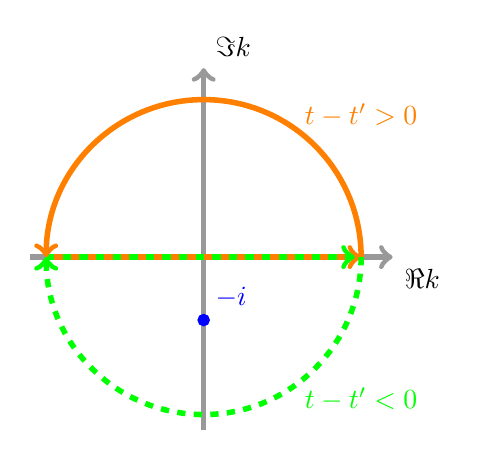
\begin{tikzpicture}  [scale=0.4]

\tikzstyle{every path}=[line width=2pt]

% Draw the axis

%\draw [color=black] (-3,0) -- (3,0);
%\draw [color=black] (0,-3) -- (0,3);
\draw[draw=gray!80,->] (0,-5) + (0,-0.5cm)  -- (0,5) -- +(0,1cm) node[above right] {$\Im k$};
\draw[draw=gray!80,->] (-5,0) +(-0.5cm,0) -- (5,0) -- +(1cm,0) node[below right] {$\Re k$};


\draw[orange,->] (-5,0) -- (5,0);
\draw[green,dashed,->] (-5,0) -- (4.8,0);

% Draw half circles

\draw [color=orange,->] (5,0) arc [start angle=0,end angle=180,x radius=5cm, y radius=5cm];
\node[orange] at (5,4.5) {$t-t'> 0$};
\draw [color=green,dashed,->] ( 5,0) arc [start angle=360,end angle=180,x radius=5cm, y radius=5cm];
\node[green] at (5,-4.5) {$t-t' < 0$};

\filldraw [color=blue] (0,-2) circle (3pt) node[above right] {$-i$};

\end{tikzpicture}
\caption{Plot of the two paths reqired for solving the Fourier integral~(\ref{2018-m-ch-gf-ip1}).}
\label{2011-m-ch-gf-fe}
\end{center}
\end{marginfigure}
}
The ``closures'' through the respective half-circle paths vanish.
The residuum theorem yields

\begin{equation}
G_1(t,t') =
\begin{cases}
0
&
\textrm{ for } t>t'\\
-2\pi i\,{\rm Res}\,\left({1\over2 \pi i} {e^{ik(t-t')}\over k+i };-i\right)= -e^{t-t'}
&
\textrm{ for } t<t'.
\end{cases}
\end{equation}
Hence we obtain a Green's function for the inhomogeneous differential equation
$$
G_1(t,t')=-H (t'-t)e^{t-t'}
$$
However, this Green's function and its associated (special) solution does
not obey the boundary conditions
$G_1(0,t')=-H (t')e^{-t'}\ne0$ for $t'\in[0,\infty)$.

Therefore, we have to fit the Green's function by adding an appropriately weighted solution to the homogeneous differential equation.
The homogeneous Green's function is found by
$
   {\cal L}_tG_0(t,t')=0$,
and thus, in particular,
${d\over dt}
   G_0=G_0\Longrightarrow G_0=ae^{t-t'}
$.
with the {\em Ansatz}
$$
G(0,t')=G_1(0,t')+G_0(0,t';a)=-H (t')e^{-t'}+ae^{-t'}  $$
for the general solution we can choose the constant coefficient $a$ so that
$$
G(0,t')=0
$$
For $a=1$,
 the Green's function and thus the solution obeys the boundary value conditions;
that is,
$$
G(t,t')=\bigl[1-H (t'-t)\bigr]    e^{t-t'}.
$$
Since $H (-x)=1-H (x)$, $G(t,t')$ can be rewritten as
$$
   G(t,t')=H (t-t')e^{t-t'}.
$$

In the final step we obtain the solution through integration of $G$ over the inhomogeneous term  $t$:
\begin{equation}
\begin{split}
   y(t)=
\int_0^\infty G(t,t')t'dt'=
\int_0^\infty \underbrace{H (t-t')}_{=1\text{ for }t'<t} e^{t-t'}t'dt'
       =\int\limits_0^t e^{t-t'}t'dt'\\=e^t\int\limits_0^t t'e^{-t'}dt'
       =e^t\left(-t'e^{-t'}\Bigr|_0^t-\int\limits_0^t(-e^{-t'})dt'
          \right) \\
       =e^t\left[(-te^{-t})-e^{-t'}\Bigr|_0^t\right]=e^t\left(
          -te^{-t}-e^{-t}+1\right)=e^t-1-t.
\end{split}
\end{equation}

It is prudent to check whether this is indeed a solution of the differential equation
satisfying the boundary conditions:
\begin{equation}
\begin{split}
{\cal L}_t  y(t)=  \left(\frac{d}{dt} -1\right) \left(e^t-1-t\right)
=e^t-1 - \left(e^t-1-t\right) =t,\\
 \textrm{and }y(0)= e^0-1-0=0
.
\end{split}
\end{equation}

%%%%%%%%%%%%%%%%%%%%%%%%%%%%%%%%%%%%%%%%%%%%%%%%%%%%%%%%%%%%%%%%%%%%%%%%%%%%%%%%%%%%%%%%%%%%%%%%

\item
Next, let us solve the differential equation
 ${d^2y\over dt^2}+y=\cos t$
on the intervall $t\in [0,\infty )$ with the boundary conditions  $y(0)=y'
 (0)=0$.

First, observe that
$
{\cal L} = {d^2 \over dt^2}+1.
$
The Fourier {\em Ansatz} for the Green's function is
\begin{equation}
\begin{split}
   G_1(t,t')={1\over2\pi}\int\limits_{-\infty}^{+\infty}
               \tilde G(k)e^{ik(t-t')}dk\\
   {\cal L}G_1={1\over2\pi}\int\limits_{-\infty}^{+\infty}
          \tilde G(k)\left({d^2\over dt^2}+1\right)e^{ik(t-t')}dk\\
       ={1\over2\pi}\int\limits_{-\infty}^{+\infty}\tilde G(k)((ik)^2+1)
          e^{ik(t-t')}dk\\
       =\delta(t-t')={1\over2\pi}\int\limits_{-\infty}^{+\infty}
          e^{ik(t-t')}dk
\end{split}
\end{equation}
Hence
$ \tilde G(k)(1-k^2)=1$
and thus
$\tilde G(k)= {1\over(1-k^2)}={-1\over(k+1)(k-1)}
$.
The Fourier transformation is
\begin{equation}
\begin{split}
    G_1(t,t')=-{1\over2\pi}\int\limits_{-\infty}^{+\infty}
                    {e^{ik(t-t')}\over(k+1)(k-1)}dk\\
                 =-{1\over 2\pi}2\pi i\left[\,{\rm Res}\left(
                    {e^{ik(t-t')}\over(k+1)(k-1)};k=1\right)\right.\\
\left.+{\rm Res}\left({e^{ik(t-t')}\over(k+1)(k-1)};k=-1\right)\right]
H (t-t')
\end{split}
\end{equation}
The path in the upper  integration plain is drawn in Fig. \ref{2011-m-ch-gf-fe2}.
{\color{black}
\begin{marginfigure}
\begin{center}
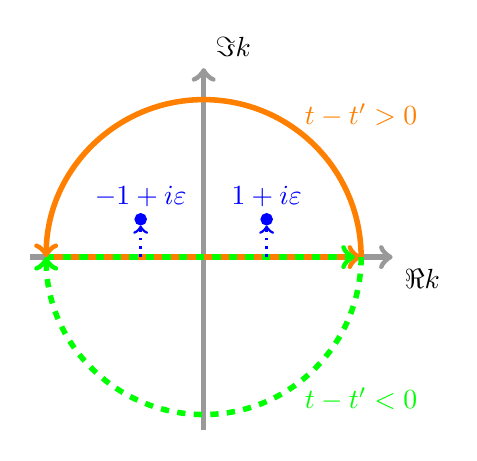
\begin{tikzpicture}  [scale=0.4]

\tikzstyle{every path}=[line width=2pt]

% Draw the axis

%\draw [color=black] (-3,0) -- (3,0);
%\draw [color=black] (0,-3) -- (0,3);
\draw[draw=gray!80,->] (0,-5) + (0,-0.5cm)  -- (0,5) -- +(0,1cm) node[above right] {$\Im k$};
\draw[draw=gray!80,->] (-5,0) +(-0.5cm,0) -- (5,0) -- +(1cm,0) node[below right] {$\Re k$};


\draw[orange,->] (-5,0) -- (5,0);
\draw[green,dashed,->] (-5,0) -- (4.8,0);

% Draw half circles

\draw [color=orange,->] (5,0) arc [start angle=0,end angle=180,x radius=5cm, y radius=5cm];
\node[orange] at (5,4.5) {$t-t'> 0$};
\draw [color=green,dashed,->] ( 5,0) arc [start angle=360,end angle=180,x radius=5cm, y radius=5cm];
\node[green] at (5,-4.5) {$t-t' < 0$};

\draw[line width=1pt,blue,dotted,->] (-2,0) -- (-2,1);
\draw[line width=1pt,blue,dotted,->] ( 2,0) -- ( 2,1);
\filldraw [color=blue] (-2,1.2) circle (3pt) node[above] {$-1+i\varepsilon$};
\filldraw [color=blue] ( 2,1.2) circle (3pt) node[above] {$ 1+i\varepsilon$};

\end{tikzpicture}
\end{center}
\caption{Plot of the   path  required for solving the Fourier integral, with the pole description of ``pushed up`` poles.}
\label{2011-m-ch-gf-fe2}
\end{marginfigure}
}
\begin{equation}
\begin{split}
   G_1(t,t')=-{i\over2}\left(e^{i(t-t')}-e^{-i(t-t')}\right)H (t-t')\\
            ={e^{i(t-t')}-e^{-i(t-t')}\over2i}H (t-t')=
               \sin(t-t')H (t-t')\\
   G_1(0,t')=\sin(-t')H (-t')=0\textrm{  since  }\quad t'>0\\
   G_1'(t,t')=\cos(t-t')H (t-t')+\underbrace{\sin(t-t')\delta(t-t')}_
                {\mbox{$=0$}}\\
   G_1'(0,t')=\cos(-t')H (-t')=0
.
\end{split}
\end{equation}
$G_1$ already satisfies the boundary conditions; hence we do not need to find the Green's function $G_0$ of the homogeneous equation.
\begin{equation}
\begin{split}
   y(t)=\int\limits_0^\infty G(t,t')f(t')dt'=
          \int\limits_0^\infty \sin(t-t')\underbrace{H  (t-t')}_
          {\mbox{$=1$ for $t>t'$}}\cos t' dt' \\
       =\int\limits_0^t\sin(t-t')\cos t' dt'=
          \int\limits_0^t(\sin t\cos t'-\cos t\sin t')\cos t' dt' \\
       =\int\limits_0^t\bigl[\sin t(\cos t')^2-\cos t\sin t'\cos t'
          \bigr]dt'=\\
       =\sin t\int\limits_0^t(\cos t')^2dt'-\cos t\int\limits_0^t
          sin t'\cos t'dt' \\
       =\sin t\left.\left[{1\over2}(t'+\sin t'\cos t')\right]\right|_0^t-
          \cos t\left.\left[{\sin^2 t'\over2}\right]\right|_0^t \\
       ={t\sin t\over2}+{\sin^2 t\cos t\over 2}-{\cos t\sin^2 t\over2}=
          {t\sin t\over2}.
\end{split}
\end{equation}


\end{enumerate}


\eexample
}

\begin{center}
{\color{olive}   \Huge
\decofourright
 %\decofourright \decofourleft
%\aldine X \decoone c
%\floweroneright
% \aldineleft ] \decosix g \leafleft
% \aldineright Y \decothreeleft f \leafNE
% \aldinesmall Z \decothreeright h \leafright
% \decofourleft a \decotwo d \starredbullet
%\decofourright
% \floweroneleft
}
\end{center}

